\documentclass[aps,prl,twocolumn,groupedaddress]{revtex4-1}
% \documentclass[aps,twocolumn,secnumarabic,balancelastpage,amsmath,amssymb,nofootinbib]{revtex4-1}
\usepackage{amsmath}
\usepackage{amssymb}
\usepackage{amsfonts}
\usepackage{color}
\usepackage{graphics}
\usepackage[pdftex]{graphicx}
\usepackage[utf8x]{inputenc}
\usepackage[colorlinks=true]{hyperref}

\newcommand{\ud}{\mathrm{d}}
\newcommand{\ue}{\mathrm{e}}
\newcommand{\ui}{\mathrm{i}}
\newcommand{\res}{\mathrm{Res}}
\newcommand{\Tr}{\mathrm{Tr}}
\newcommand{\dsum}{\displaystyle\sum}
\newcommand{\dprod}{\displaystyle\prod}
\newcommand{\dlim}{\displaystyle\lim}
\newcommand{\dint}{\displaystyle\int}
\newcommand{\fsno}[1]{{\!\not\!{#1}}}
\newcommand{\texp}[2]{\ensuremath{{#1}\times10^{#2}}}
\newcommand{\dexp}[2]{\ensuremath{{#1}\cdot10^{#2}}}
\newcommand{\eval}[2]{{\left.{#1}\right|_{#2}}}
\newcommand{\paren}[1]{{\left({#1}\right)}}
\newcommand{\lparen}[1]{{\left({#1}\right.}}
\newcommand{\rparen}[1]{{\left.{#1}\right)}}
\newcommand{\abs}[1]{{\left|{#1}\right|}}
\newcommand{\sqr}[1]{{\left[{#1}\right]}}
\newcommand{\crly}[1]{{\left\{{#1}\right\}}}
\newcommand{\angl}[1]{{\left\langle{#1}\right\rangle}}
\newcommand{\tpdiff}[4][{}]{{\paren{\frac{\partial^{#1} {#2}}{\partial {#3}{}^{#1}}}_{#4}}}
\newcommand{\tpsdiff}[4][{}]{{\paren{\frac{\partial^{#1}}{\partial {#3}{}^{#1}}{#2}}_{#4}}}
\newcommand{\pdiff}[3][{}]{{\frac{\partial^{#1} {#2}}{\partial {#3}{}^{#1}}}}
\newcommand{\diff}[3][{}]{{\frac{\ud^{#1} {#2}}{\ud {#3}{}^{#1}}}}
\newcommand{\psdiff}[3][{}]{{\frac{\partial^{#1}}{\partial {#3}{}^{#1}} {#2}}}
\newcommand{\sdiff}[3][{}]{{\frac{\ud^{#1}}{\ud {#3}{}^{#1}} {#2}}}
\newcommand{\tpddiff}[4][{}]{{\left(\dfrac{\partial^{#1} {#2}}{\partial {#3}{}^{#1}}\right)_{#4}}}
\newcommand{\tpsddiff}[4][{}]{{\paren{\dfrac{\partial^{#1}}{\partial {#3}{}^{#1}}{#2}}_{#4}}}
\newcommand{\pddiff}[3][{}]{{\dfrac{\partial^{#1} {#2}}{\partial {#3}{}^{#1}}}}
\newcommand{\ddiff}[3][{}]{{\dfrac{\ud^{#1} {#2}}{\ud {#3}{}^{#1}}}}
\newcommand{\psddiff}[3][{}]{{\frac{\partial^{#1}}{\partial{}^{#1} {#3}} {#2}}}
\newcommand{\sddiff}[3][{}]{{\frac{\ud^{#1}}{\ud {#3}{}^{#1}} {#2}}}
\newcommand{\eff}{ef\! f}
\newcommand{\fxnote}[1]{{\textbf{[#1]}}}

\newcommand{\todo}[1]{}

\ifpdf
% Ensure reproducible output
\pdfinfoomitdate=1
\pdfsuppressptexinfo=-1
\pdftrailerid{}
\hypersetup{
  pdfcreator={},
  pdfproducer={}
}
\fi

\begin{document}
\title{Coherent optical association of a single molecule}
\author{Yichao Yu}
\email{yichaoyu@g.harvard.edu}
\author{Kenneth Wang}
\author{J. D. Hood}
\author{Lewis Picard}
\author{Jessie T. Zhang}
\author{William Cairncross}
\author{Jeremy Hutson}
\author{Till Rosenband}
\author{Kang-Kuen Ni}
\email{ni@chemistry.harvard.edu}
\affiliation{Department of Chemistry and Chemical Biology, Harvard University, Cambridge, Massachusetts, 02138, USA}
\affiliation{Department of Physics, Harvard University, Cambridge, Massachusetts, 02138, USA}
\affiliation{Harvard-MIT Center for Ultracold Atoms, Cambridge, Massachusetts, 02138, USA}

\date{\today}

\begin{abstract}
  We report on coherent association of a single weakly-bound NaCs molecule in an optical tweezer
  through an optical Raman transition without the use of a Feshbach resonance. Our scheme borrows transition dipole moment while reducing photon scattering by selecting a deeply bound electronic excited intermediate state.
  Starting from two atoms in their relative motional ground state,
  we achieve optical transfer efficiency of $50 \%$ \todo{number}.
  The molecule has a (change to 8.8G) zero-field binding energy of $770 \mathrm{MHz}$ \todo{number}
  and lifetime up to $1 \mathrm{ms}$ \todo{number}. (center of mass motional state population.)
  % We demonstrate that coherent creation of a ground-state single molecule is possible, even without Feshbach resonance or narrow optical transition.
  This  technique is general (does not rely on narrow excited state linewidth) and could allow a wider range of molecular species to be assembled atom-by-atom.
\end{abstract}

% Coherent
% Intermediate state
% Motional state control
% Initial state preparation

\maketitle

% Introduction


% 1. we want to have a diverse species to tailor to different applications including precision measurements and quantum engineering. 2. for the technique of associating atoms to form molecules, but so far all has been done with Feshbach association (before STIRAP), or in the case of Sr2, a narrow excited state. Previous work on near-threshold Raman transfer has been incoherent.
%(suggested referees: Florian Shreck and Immanual Bloch, Tanya, Deep Gupta, DeMille)

%Trapped neutral molecules, assembled in an array of optical tweezers, are a promising platform to study quantum information and quantum simulation. (more detail to add here about applications?).

Diverse species of fully quantum controlled  ultracold molecules are desired for a  wide variety of applications including precision measurements~\cite{Nick_and_Ivan2017}, quantum simulations~\cite{Yao2018}, quantum  information processing~\cite{DeMille2002, Ni2018}, and studies of ultracold chemistry.
While many innovative approaches demonstrated in the last few years have directly cooled different species of diatomic or polyatomic molecules  below 1~mK~\cite{Norrgard2016}, the coldest and the highest phase-space-density gas to date in an ensemble~\cite{Demarco2018} or as individuals~\cite{Zhang2020}  have been achieved through the associations of ultracold atoms.
%(any place to cite  molecular ion work?)
% cite recent doyle group result on cooling symmetric top molecule? FOR SURE, and other laser cooling works and electro-optical-cooling! Citations are not complete. Add them as you see fit.

Such ultracold molecular association takes advantage of the much developed cooling and trapping techniques for atoms  as a starting point. To overcome the challenges of small wavefunction overlap and the large release of binding energy of converting atoms to deeply-bound molecules, a  two-step approach have been established to first associate atom pairs into weakly-bound molecules, and then transfer the molecules from one internal state  to a desired rovibrational and electronic state~\cite{Danzl2008, Ni2008,Lang2008, Takekoshi2014, Molony2014, Park2015, Guo2016, Kondov2019, Voges2020}.
So far, all of such association process  utilize a magnetic Feshbach scattering resonance and  apply to bialkali molecules. The only exception is Sr$_2$~\cite{Reinaudi2012,Stellmer2012} where narrow linewidth excited states are available and optical association can be driven. The requirement of a Feshbach resonance to enhance atom-to-molecule wavefunction overlap or the narrow excited state lines limits the generality of the association technique to more diverse molecular species. 


Here, we demonstrate coherent association of an atom pair to a weakly bound molecule using an optical Raman transfer via an electronic excited state, without the use of a Feshbach resonance nor a narrow excited state. Our scheme is based on theoretically determined most suitable vibrational state of the electronic excited state $c^3\Sigma^+$ that balances transfer coupling and photon scattering. Furthermore, to reduce technical requirements such as intensity stability, etc , we choose a initial and final state ... This approach is general and can be use to associate other molecular species or large molecules atom-by-atom.
%electronic the best initial hyperfine combination of the atoms to use and best single photon frequency that balances coupling/transfer efficiency and photon scattering. Using these parameters, we demonstrate coherent association of a electronic ground-state molecule from two atoms via an optical Raman transition in an optical tweezer.




%Production of ultracold molecules in optical tweezers is challenging due to their internal degrees of freedom including rotation and vibration. In certain molecular species with relatively closed cycling transitions, direct laser cooling remains a viable option. However, for many species, including NaCs, the vibrational branching ratios are unfavorable, making direct laser cooling challenging. In these systems, a bottom-up approach of assembling the molecule from its constituent atoms has been demonstrated both in bulk gas and in optical tweezers. The challenge in a bottom-up approach is the vastly different length scales between the free atoms and a ground state molecule, leading to small coupling between them. For atoms in the motional ground state in the tweezer, the average distance between the two atoms is about $1000a_0$. However, for the ground rovibrational molecule, the bond length is only around $4a_0$. Because of this, it is necessary to use an intermediate state with a size in between the initial and final states, and accomplish the transfer in two steps in order to increase the coupling.

%The traditional choice for such an intermediate state is a weakly-bound Feshbach molecule, which can be coherently produced by ramping a magnetic field across the Feshbach resonance \todo{cite our FB result}. However, this requires a suitable Feshbach resonance, which limits the generality of this technique. An alternative approach uses a weakly bound ground electronic molecular state as the intermediate state (I'm wondering how we can distinguish this weakly bound molecular state from the weakly-bound Feshbach molecule state, we can maybe specify typcial binding energies? "most weakly bound state of the low field ground state electronic potential" maybe?), populated by an optical Raman transition, schematically shown in figure \todo{}. In this scheme, a pair of Raman beams is used to drive the unbound, but confined, atoms to a bound molecular state via an excited molecular state. This approach minimizes the reliance on system specific properties and can therefore be more generally applied to creating other molecules. Such a transfer using an optical transition has been observed in previous experiments \todo{cite}. However, they either require the use of a narrow optical transition which limits the generality or were driving the transition incoherently due to scattering.

% the requirement of a suitable FB resonance limits its generality. \todo{e.g. non-magnetic atoms?}

% The size mismatch between the initial and final states cause a very small coupling between them,
% which poses the biggest challenge for for coherent creation of the molecule.




% Because the electronic excited state we used are generic in most diatomic molecules, this technique is general....


\begin{figure*}
  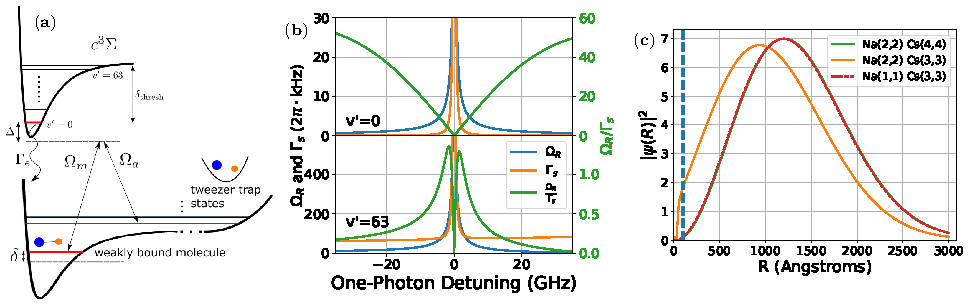
\includegraphics[height=5cm]{fig1.pdf}
  \caption{Optical creation of single molecule from single atoms in tweezer.
    (A) Schematics of the Raman transition. \todo{more about the states involved}
    (B) Geometry and polarization of trap and Raman beam relative to the bias magnetic field.
    \todo{Field strength, power, polarization description (pi)}
    (C) Molecule formation pulse sequence. The tweezer initially consists of only up leg power.
    This power is smoothly ramped down and the down leg power ramped up over $10\mu s$ while
    maintaining the total power of the tweezer.
    \todo{to minimize heating?}
    \label{f-setup}
  }
\end{figure*}

\begin{figure*}
  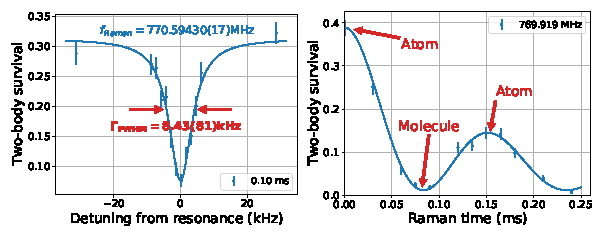
\includegraphics[height=4.5cm]{fig2.pdf}
  \caption{
    (A) Raman resonance from atomic state to molecular state, showing Fourier limited linewidth.
    \todo{states, time}
    (B) Rabi oscillation on resonance
    \label{f-raman}}
\end{figure*}

\begin{figure*}
  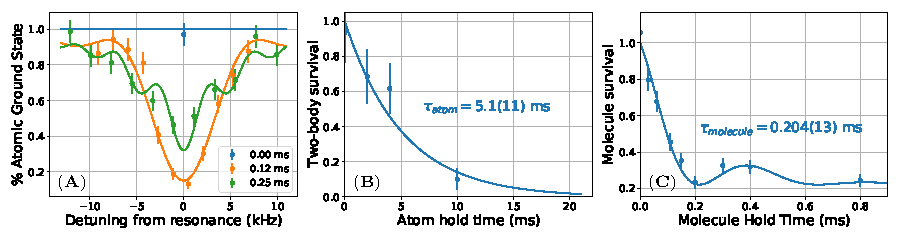
\includegraphics[height=4.5cm]{fig3.pdf}
  \caption{
    (A) Two-body atom lifetime in 15 mW of trap depth \todo{lifetime number,
      subtraction of single body, photoassociation rate}
    (B) Molecule lifetime in 15 mW of trap depth \todo{lifetime number}
    \label{f-lifetime}}
\end{figure*}

\begin{figure*}
  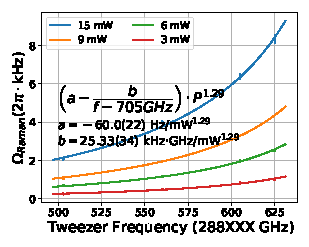
\includegraphics[height=4.5cm]{fig4.pdf}
  \caption{Raman Rabi frequency vs detuning
    \label{f-det}}
\end{figure*}




% In this letter, we will present our result on coherent creation of a weakly bond molecule
% using only optical transitions on a broad optical line for the first time.


% The optical transfer scheme we use is shown in figure \todo{}. To drive the atoms from
% We use an optical Raman transition to drive the system from the atomic initial state to a ground electronic molecular state. In order to reduce the size mismatch between the atomic and molecular states, we selected the first bound state for the 3322 spin state \todo{asymtopt to the 3322 threshold?} as our final state. \todo{move selection of intermediate state to intro?}. For similar reason, the natural choice for the intermediate excited molecular state is one with highly excited motional level.However, from our calculation (and experiment?), the smaller level space for high vibrational state and the smaller detuning from the atomic threshold increases the scattering rate of the molecular state which causes a reduced Raman Rabi frequency to decoherence rate ratio and a lower transfer efficiency. Therefore, in our experiment, we selected the v=0 state as the intermediate state for our Raman transition.

While optical Raman transfer of atoms to molecules utilizing an electronic excited state has been shown previously\todo{cite}. Those demonstrations were  incoherent  where the signal comes from loss of population (and therefore more like spectroscopy and the transferred molecules cannot be further utilized). The challenge lies at  achieve high enough Raman Rabi frequency to drive this transition due to the wavefunction size mismatch with the excited molecular state.
 Previous experiments use weakly bound molecular excited states in the Raman transition to increase the Raman Rabi frequency. However, this choice of state also increases the scattering during the transfer process for two reasons.
Firstly, since for a typical molecular potential the spacing between states
decreases with increasing vibrational levels,
a weakly bound excited molecular state limits maximum usable detuning and therefore the effectiveness of scattering reduction by increasing the detuning for the Raman transition.
Secondly, due to size similarity, the weakly bound molecular ground state has a strong coupling with the atomic excited state which contributes significantly to the total scattering rate.
The rate of such scattering process is proportional to $1/\delta_{thresh}^2$,
where $\delta_{thresh}$ is the detuning from the dissociation threshold. (Should we also mention scattering of the atomic initial state too? This should affect the Raman process as well)
% This further increases the scattering rate for a weakly bond excited state.
Based on these considerations, we calculated both the Raman Rabi frequency and the scattering rate at different detunings. As seen in figure (1....), despite a higher Raman Rabi frequency at the same detuning, using a weakly bound intermediate state results in a much higher scattering rate and ultimately a smaller Rabi frequency to scattering rate ratio as compared to deeply bound states. As a result, we use a deeply bound molecular excited state to drive the Raman transition.

%(goes to SM?)

(mention scattering/lightshift depends on up/down matrix element ratio?)

In addition to the intermediate state, the choice of the initial and final states are critical for both fundamental and technical reasons. A key difference in molecular association via a Raman process compared to Raman transfer between hyperfine states in atoms is that the matrix elements between the ground states and the excited state are greatly unbalanced. In particular, the matrix element between the molecule state and the excited state, $ \Omega_m $ is much larger than the matrix element between the free atom state and the excited state, $ \Omega_a $. To understand the effect of this inbalance, we consider a 3 level model, and ignore the presence of multiple excited states. The Raman Rabi Rate, $ \Omega_a\Omega_m / 2\Delta$ depends on both matrix elements, but the scattering rate predominantly comes from the final molecular state, $ \Gamma_e \Omega_m^2 / 2\Delta^2$, where $ \Gamma_e $ is the excited state linewidth and $ \Delta $ is the single photon detuning. Assuming the power of each Raman beam is equal, there is an additional factor of 2 in the scattering rate, since the molecular state scatters off of both Raman beams at roughly the same single photon detuning. Thus, the ratio between the Raman Rabi frequency and the scattering rate, $ \Omega_a/\Omega_m \times \Delta/\Gamma_e $, depends on the ratio of the two matrix elements and how far detuned the laser is from the transition in units of the linewidth. Thus, a small $ \Omega_m/\Omega_a $ ratio is desired to be able to drive this transition coherently. In addition to this fundamental reason, there is also a technical advantage for having a $ \Omega_m/\Omega_a $ ratio to be as small(? or big) as possible. The position of the resonance depends on the laser power predominantly through the AC Stark shift on the molecular state, $ \Omega_m^2 / 2\Delta $. The ratio of the AC Stark shift to the Raman Rabi frequency is $ \Omega_m / \Omega_a $, Thus, the laser needs to be stabilized to better than the inverse of this ratio, $ \Omega_a/\Omega_m $, to fluctuate by less than a linewidth. This becomes technically easier when $ \Omega_m/\Omega_a $ is smaller. 
(for our choice of states, this mean intensity fluctuation of less than 1\% or 0.1\%.)

Due to the small size of the molecular wavefunction, the coupling between the ground atomic state and the excited molecular state is approximately proportional to the value of the relative atomic wavefunction at short distance within the molecular potential. In additional to the confinement, this value is related to the interaction between the two atoms. For states with a large scattering length (positive or negative), the phase shift in the relative wavefunction between the atoms can significantly increase the short range wavefunction (add figure?). The increase in the coupling is proportional to (quote/cite Olive's equation?). For our system, among the stable spin combinations, 4422 and 3311 has a small scattering length of $\abs{a}=....$ respectively and 3322 has a large and negative scattering length. (interaction shift $\approx$ binding?) Thus, we use the 3322 spin combination as our initial state and drive to the first bound state for the 3322 spin combination.

% In additional to the final and the excited state, it is also important to select the an initial atomic state in order to improve the coupling.


%% Preparation
Our experiment begins by loading a single ${}^{23}\mathrm{Na}$ atom and a single ${}^{133}\mathrm{Cs}$ atom into an optical tweezer from a dual-species MOT\todo{cite na loading paper} into separate optical tweezers. The atoms are imaged to distinguish between loading of two atoms, one atom (Na or Cs), or no atom during post selection. We then perform simultaneous Raman sideband cooling (RSC) to cool both atoms into the 3-dimensional motional ground state of their optical tweezers. After RSC, the Na tweezer is moved by sweeping the frequency on an acoustical optical beam deflector (AOBD) to overlap with the Cs tweezer before smoothly ramping off rso that the Na and Cs atoms are merged into the same tweezer \todo{cite}. The spin states for the Na and Cs atoms after RSC and during the merge process are $|F=2,m_F=2\rangle$ and $|F=4,m_F=4\rangle$ respectively. This states combination has a low scattering length of $... a_0$ which allows the two atoms to be merged into the same tweezer with minimum pertubation on each other and thus they remain in the motional ground state after the merge.

After preparing the Na and Cs atoms in the same tweezer in a single quantum state, we need to drive the atoms into the large scattering length 3322 hyperfine combination. To do this, we perform interaction shift spectroscopy using a Cs Raman transition to drive the Cs into the $|F=3,m_F=3\rangle$ state (Is this really "performing spectroscopy"? Or should we just say we drive a Raman transfer to flip the spin). The new spin state combination has a larger scattering length of $... a_0$ which generates a interaction shift of $... kHz$ in the tweezer. This interaction shift is larger than the differential axial trapping frequency between Na and Cs atoms, which decouples the relative and center of mass motional state and improves the robustness of our preparation of relative motional ground state.

% The stronger interaction in this spin state also enhances the atomic wavefunction at short range and increases its overlap with the intermediate molecular state used for our Raman transfer..

%% Transfer scheme
After the atoms are prepared in the 3322 hyperfine combination, we then perform the Raman transfer. The pulse sequence for this step is shown in figure (). Instead of adding another beam to drive the Raman transition on the atoms in the tweezer, we use the tweezer itself to achieve this goal. The dual use of the tweezer beam ensures that there is not any undesired laser frequency that can interfere with the Raman transition, and also allows us to maximize the Raman Rabi frequency and minimize the transfer time (also minimize source of scattering). After the total tweezer power is set to the desired value, we smoothly ramp down the power of one frequency in the tweezer while simultaneously ramping up the power of a different frequency so that the total tweezer power remains unchanged. Both frequencies are kept on for a variable length of time before the process is reversed and we return to having a single frequency in the tweezer.
\todo{clarify coprop of Raman beam?}

%% Experiment condition/resonance

We locate the Raman resonance for the atom to molecule transition at $770... MHz$ (figure \todo{}) with a $15 mW$ tweezer at $288... GHz$ which corresponds to a $... GHz$ single photon detuning. (We can maybe add information about the prediction here?)
%% Prediction
% This excited state used in the Raman transition was measured in our previous experiment using photoassociation to be at $288... GHz$ from our atomic state. The ground molecular state has not been observed previously in experimentally. Based on our measurement of FB resonance, interaction shift and the binding energy of the 4422 bound state. Theory prediction was at $770... MHz$. \todo{more, mention/cite Jeremy}
The background level of $...\%$ corresponds to the probability of preparing the two atoms in the relative motional ground state using interaction shift spectroscopy (can this be considered "interaction shift spectroscopy"?). When the atoms are transferred into the molecule state by the Raman transition, there is a decrease in the two body survival since the resulting molecule is not directly detected by our imaging step.
We observed the narrowest linewidth of $.... kHz$ for the Raman resonance at a pulse time of $... ms$, which corresponds to a linewidth-pulsetime product of $...$. This is consistent with the expected value of $...$ for an ideal $\pi$ pulse which is an evidence that the transfer is coherent. In order to verify the coherence of the transfer directly, we fixed the Raman frequency on the resonance and scanned the pulse time. figure ... shows the observed Rabi oscillation between the atomic and molecular states. Fitting the data with a decaying Rabi oscillation suggests that $..\%$ of initial ground state atoms are transfered into the molecular state.

In order to understand the fidelity of molecule formation, we fit our measurements to a model that includes a Raman Rabi frequency and a finite lifetime for the final molecular state (figure 3...). The effect due to atomic state loss was taken into account by measuring the single and two body lifetime of the atoms directly (figure 3...). The fit shows that we have a Raman Rabi frequency of $...$. The molecule we form has a lifetime of $...$ which is the main limitation on the fidelity of the transfer. The molecule lifetime can be verified directly by adding a second Raman pulse to dissociate the molecule back to atoms after a variable wait time (figure 3...). The result shows a molecular lifetime consistent with our fitting of the Raman transition data.

The ratio of molecule scattering rate and the Rabi frequency is larger than the theory prediction.
In order to understand the origin of this discrepancy, we measured the dependency of the Raman resonance as a function of the tweezer power and frequency. The important results from the fits are resonance frequency (light shift), Raman Rabi frequency, atomic lifetime and molecular lifetime, each provide us information about a different combination of physical processes.

First we look at the change in resonance frequency. As a function of the tweezer power, we observed a linear dependency on the resonance frequency caused by the differential light shift between the atomic and molecular state (figure ?). When we vary the tweezer frequency around the $v=0$ excited state, we can further observe a $1/\delta$ component and a background component that is constant for different detunings. The background is caused by coupling to all the other excited states that are further away which is not very important in this case. The $1/\delta$ component, however, is due to the coupling to the $v=0$ excited state and from equation (?) we know that this is mainly due to the coupling between the excited and ground molecular states. From this, we can calculate a down leg matrix element of $....$ which is similar to what we calculated from theory (ref/sm theory). (make sure theory part mentions $\Omega_{down}\gg\Omega_{up}$, also $\Omega$ vs $\Omega'$ for the single leg vs cross coupling number).

(talk about blue side?)

The Raman Rabi frequency shows a non-linear dependency on the tweezer power due to the change in the atomic wavefunction caused by the change in confinement. The up leg matrix element scales with the short length atomic wavefunction amplitude which is 0.375 for weakly interaction particles. However, due to the strong interaction between the two atoms, this approximation breaks down. Instead, theory calculation shows that the scaling is very well approximated by a power of 0.29 within the range of confinement in our experiment. Combined with the intensity factor of the Raman beams, the Raman Rabi frequency should scale with 1.29 power of the tweezer intensity, which agrees with our experimental result. Similar to the light shift, there is also a background component and a $v=0$ component in the Raman Rabi frequency. The $v=0$ component predicts a up leg Rabi frequency of $...$ which is consistent with theory. Unfortunately, the background Raman Rabi frequency cancels the Rabi frequency for red detuning Raman transition which is one of the factors that decreases our transfer efficiency. (need blue side?)

Next, we look at the atomic loss rate during the transfer process.
The atomic loss rate scales as the tweezer intensity to the 2.58th power but shows little to no dependency on the tweezer frequency. The lack of frequency dependency suggests that most of the atomic loss are due to the coupling to states other than the $v=0$ one. After substracing 0.58 from the power scaling due to the change in the up leg matrix element, the loss rate is proportional to the tweezer power squared. This is an evidence that the loss is likely caused by a two photon scattering process rather than one photon scattering. The strong power scaling causes a faster than expected loss rate for the atom. However, the atomic scattering is contribution only a small fraction of the total scattering rate so this is not the limiting factor for the transfer.

Finally, we fit the scaling for the molecular loss rate. We observed a dependency on the detuning that is consistent with $1/\delta^2$ suggesting that the loss is indeed mostly coming from the $v=0$ excited state. (preliminary) We observed a power scaling power of $\approx1.2$ which is closed to the prediction for a single photon scattering process. The excited state line width calculated from the scattering rate is $...(1 GHz?)$ which is much larger than the theory prediction of $10 MHz$ as well as the $20 MHz$ upper bound from our previous PA measurements (cite).

(ASE filter)

%%%% Maybe this following section about the B field can be relegated to a figure caption?
% Figure () shows the geometry of the experiment setup. A $8.8\mathrm{G}$ B field was used to defines the quantization axis in the experiment and is applied perpendicular to the tweezer axis. The tweezer beam (both frequencies for the Raman transition) has a $\pi$ polarization relative to the quantization axis, which allows us to selectively drive the Raman transition to a final state with the same total $m_F$ quantum number as our initial state.








B field dependency $... kHz/G$ which agrees with theory prediction of $... kHz/G$.
Dependency on tweezer power $... kHz/mW$, extrapulated to obtain the bare resonance at $0$ tweezer power to be at $... MHz$.

\todo{sm: STIRAP vs Raman}

%\bibliography{paper}
\bibliography{master_ref}
\bibliographystyle{apsrev4-2}
\end{document}
